\acresetall
\chapter{Principled Operationalisation using Presage2}\label{ch:presage}

\lettrine[lines=3]{P}{rincipled} Operationalisation is the process of transforming a symbolic or formal representation of a system (often written in some kind of calculus) into a computer model of the system in question~\citep{Jones2013}. This process varies greatly in difficulty depending on the complexity of the system to be modelled and the requirements of the computer model. Models can range from small prolog programs~\citep{Pitt2005a} to significant software engineering undertakings~\citep{Timm,Oguara2005}.

\ac{ABM} and \ac{MABS} are approaches to modelling and simulating complex systems as multi-agent systems~\citep{Macal2010,Moss2001}.
This is a form of micro-simulation, where by modelling low-level interactions from the `ground up' we can observe macro level behaviours such as self-organisation, self-adaptation and so on.
Simulation models are therefore composed of an environment or arena which models the behaviour of a physical or virtual world, and autonomous, intelligent `agents' who interact with this world and other agents. 
\citet{Axelrod1997} identifies the usefulness of \ac{MABS} as a means to understand social systems. 
This approach fits naturally to the principled operationalisation phase of the \ac{SIC} methodology, as we are observing desirable macro level performance in social systems (which are multi-agent in nature), and aiming to reproduce this performance in a socio-technical system. 

It should be noted that principled operationalisation, \ac{ABM} and \ac{MABS} do not aim to create an exact model of a social or socio-technical system, particularly in regards to human behaviour. Both the \ac{SIC} methodology and \ac{MABS} methods stress the appropriate use of abstraction and/or compartmentalisation in order to simplify the model while being able to draw valid conclusions from the model's behaviour~\citep{Edmonds2001}.

Work in \ac{ABM} and \ac{MABS} has led to creation of many software packages and platforms to ease the development of simulation testbeds~\citep{CynthiaNikolaiandGregoryMadey2009}. These aim to reduce the engineering effort required to implement agent models, providing reusable components, user-interface based design and/or prescriptive frameworks. In particular, they aim to ensure simulation validity while maintaining usability and extendibility~\citep{Axelrod1997}.

In this chapter we derive a set of requirements for a general-purpose software platform for simulation of socio-technical systems, which is suitable for principled operationalisation. We then review a selection of existing platforms with respect to these requirements, concluding that building upon our existing Presage platform~\citep{Neville:2009} best meets our needs. Finally we present the result of this work, Presage2~\citep{Macbeth2014}. % TODO

%\section{Requirements}
%
%\begin{itemize}
%\item Heterogeneous agents
%\item Full agent architectures
%\item Inter-agent communication
%\end{itemize}

\section{Review of Software Platforms for Agent-based Simulation}

There are many software tools and platforms available for the simulation of agent societies: A comprehensive survey by \citet{CynthiaNikolaiandGregoryMadey2009} includes 53 different toolkits. In this section we discuss the state of the art of \ac{MABS} toolkits and software platforms.

The afore-mentioned survey by \citet{CynthiaNikolaiandGregoryMadey2009} is an exhaustive survey of platforms documenting programming languages, software licenses, targeted research domains, presence of tutorials and support, and more for each platform. There are several other more focused reviews of simulation platforms: \citet{Railsback2006} describes and compares the implementation of several, gradually increasing complexity, models on four platforms, Netlogo, MASON, Repast and Swarm. \citet{Castle2006} reviews six platforms (Swarm, MASON, Repast, Starlogo, Netlogo and OBEUS) with a particular focus on geospatial simulations. \citet{Tobias2004} compares four platforms for `social-scientific' agent-based simulation (Repast, Swarm, Quicksilver and VSEit).

There are several reasons for using specific software tools for \ac{ABM} and \ac{MABS}, rather than bespoke software:
\begin{itemize}
\item \emph{Tools for non-programmers}---The inter-disciplinary nature of \ac{ABM} means than for many researchers software development is a major obstacle in adopting \ac{MABS}. Platforms can simplify model and agent implementation and hide complex implementation details, allowing more researchers to be able to understand and implement models without software engineering skills.
\item \emph{Rapid-prototyping}---The use of a platform precludes the need for work implementing and testing simulation control code when writing a software model. This time can be used for model implementation from the start, thus allowing researchers to very quickly of from ideas to working prototypes running in a simulation.
\item \emph{Code re-use}---An established platform providing a uniform base for the implementation of models and agent algorithm should allow for the porting of these implementations to other models and simulations. This enables collaboration as ideas can easily be adopted and compared without having to rewrite code.
\item \emph{High performance simulations}---Optimisation of simulations is a research area in its own right. Thus it is unrealistic to expect modellers to be able to write their own simulation software \emph{and} optimise it. The use of simulation platforms allows users to benefit from faster simulation performance.
\item \emph{Validation and verification}---Software engineering is an error prone activity. Using a known and peer-reviewed simulation platform affords some level of trust that this component should work correctly and not introduce false results. 
\end{itemize}

In this section we firstly derive a set of requirements and comparative criteria for agent-based simulation platforms. Using this we review a set of candidate platforms for principled operationalisation. 

\subsection{Requirements and Comparative Criteria}

% TODO paragraph test against software tool reasons + socio-technical reqs + principled op reqs.
We derive a set of review criteria based on a selection of relevant criteria from the previous reviews.

From~\citet{CynthiaNikolaiandGregoryMadey2009} we take generial criteria which affect platform uptake, usability and verifiability:

\begin{itemize}
\item Programming Language---The programming language required to use a platform has an affect on user uptake, quality of available development tools, code readability and succinctness, and ease of debugging~\citep{Railsback2006}. Use of custom programming languages my appear to limit the possible models which can be implemented on the platform, while general-purpose languages such as Java have known capabilities. These languages also come with a rich array of development suites to choose from to ease the development process.
\item Software License---Open source licenses are preferable as they allow the platform's code to be scrutinised, allowing both users and reviewers to verify that simulation output will be correct.
\end{itemize}

\citet{Castle2006} identifies criteria for ease-of-use:

\begin{itemize}
\item Required programming experience---Expertise needed in general programming and/or the language of the platform in order to correctly use the software.
\item Integrated charting/graphing/statistics---Whether graphical tools for data analysis during and after simulation are provided.
\item Tutorials/Documentation available---Presence of tutorials and documentation to allow one to train oneself to use the platform correctly and proficiently.
\end{itemize}

\citet{Tobias2004} provides several useful general criteria and criteria specific for the modelling requirements of socio-technical systems:

\begin{itemize}
\item Support for modelling---\ac{GUI} or other tools for reducing programming work and visualising output.
\item Support for experimentation---Tools for generation of simulations and data recording.
\item Large number of complex agents---The ability of the platform to efficiency run complex agents to intensive reasoning.
\item Inter-agent communication---The possibility of sending messages between agents, and for communication network topologies to be simulated.
\item Generating agent populations---Automatic generation of agent populations from input parameters or data.
\item Generating networks---Automatic generation of networks based on various characteristics.
\item Management of spatial arrangements---Ability to simulation situated agents.
\item Dynamically changing model structure---Whether the model can be changed during simulation execution.
\end{itemize}

We also add a final criterion specific to the principled operationalisation process:
\begin{itemize}
\item Rule engine---Executable specifications~\citep{Artikis2010} are formal characterisations where the calculus can be directly run as a computer model. These characterisations are declarative in nature, thus with a rule engine we can improve the speed and accuracy of principled operationalisation by directly integrating them into the simulation.
\end{itemize}

\subsection{Reviewed Platforms}

We will now review four software platforms with respect to the criteria we identified. These platforms are:
\begin{itemize}
\item Netlogo~\citep{Wilensky1999a}---This is a \ac{GUI}-driven modelling environment for simulating natural and social phenomena, aimed at ease of use for non-programmers. It uses a custom programming language for the specification of the environment and agent behaviours.
%\item JADE~\citep{Bellifemine2003}---This is a middleware for multi-agent system deployment which can also be used for simulation. It uses an agent model tied very closely to the FIPA agent communication specification\footnote{http://www.fipa.org}, and lacks support for modelling of the agents' environment.
\item Repast~\citep{Collier2009}---This is a familty of platforms created at the University of Chicago, originally based on the SWARM platform~\citep{Minar1996}. For this review we will look at their Java-based platform, Repast Simphony, which has superseded their other tools.
\item MASON~\citep{Luke2005}---This is a newer, discrete event, platform developed at George Mason University written in Java, and focusing on simulation execution speed.
\item Presage~\citep{Neville:2009}---This platform is a recent development, and therefore does not appear in reviews. It was developed specifically for simulation of social networks and dynamics but has found use in an array of other \ac{MABS} applications~\citep{Pitt2011,Carr2012} and features a strong animation and visualisation component.
\end{itemize}

% Notable omissions: SWARM and JADE

\autoref{tab:platformreview} shows the platforms rated according to the criteria we selected from \citet{CynthiaNikolaiandGregoryMadey2009} and \citet{Castle2006}. We will now discuss the remaining criteria:

\begin{table}[!h]
\begin{minipage}{1\textwidth}
	\myfloatalign
	\caption{Evaluation of simulation platform according to review criteria}\label{tab:platformreview}
	\begin{tabularx}{\textwidth}{X|p{0.12\textwidth}p{0.12\textwidth}p{0.12\textwidth}p{0.12\textwidth}}
	Criterion & Netlogo & Repast & Mason & Presage \\ \midrule
	Programming Language & Netlogo & Java & Java & Java \\
	Software License & Closed source & BSD\footnote{Berkeley Software Distribution licence: A permissive free software licence. Not compatible with the \ac{GPL}} & AFL\footnote{Academic Free License: A permissive free software licence. Not compatible with the \ac{GPL}} & Closed source \\
	Required programming experience & Basic & Strong & Strong & Strong \\
	Integrated graphics & Yes & Yes & None & Some \\
	Tutorials / Documentation & Yes & Yes & Yes & No \\
	\end{tabularx}
\end{minipage}
\end{table}

\subsubsection*{Support for modelling}

This is the extent to which the platform speeds up common modelling tasks, for example by providing simple \ac{GUI}-based design and/or simple visualisation tools.

Being primarily \ac{GUI}-based, and including environment and graphing visualisation as standard, Netlogo performs well in this criterion. Similarly Repast has some \ac{GUI} tools, but still requires the majority of functionality to be implemented in code. The remaining platforms do provide helper classes for common tasks, but these still require implementation with code.

\subsubsection*{Support for experimentation}

This is how well the platform supports experimentation over multiple simulations to test parameter spaces. All platforms support parameterisation of simulation runs, however MASON and Presage lack the ability to automatically generate experiments consisting of a series of simulation runs.

\subsubsection*{Large number of complex agents}

None of the platforms impose a hard constraint on the number of agents in a simulation, though depending on the efficiency of the software, practical limits will be reached when either computational resources are exhausted, or the simulation takes too long to run.

Netlogo's simulation times have been shown to scale more with the size of the environment state to be modelled, while Repast and MASON scales with the number of agents~\citep{Railsback2006}.  However the agent models tested were fairly basic. More complex agent architectures are likely to be impossible in Repast. MASON is designed with the intention of accommodating complex agents by being fast and lightweight. Similarly Presage has been demonstrated simulating complex agents~\citep{Pitt2011}.

All but one of the platforms run their main simulation in a single thread. Repast uses a multi-threaded discrete-event scheduler to run some events in parallel, however this performance boost is only available to certain background tasks, and not appropriate for agent execution. MASON also allows for some parallelisation within a simulation step, which the users must add themselves. Thus these simulators have limited capabilities to exploit modern, multi-core processors.

There is, however, more options for scaling simulations to distributed architectures. The Repast developers also distribute a C++ platform for \ac{HPC} clusters~\citep{Collier2013}, but this is separate from the Java platform. There have also been several attempts to provide an automatic scaling of normal Repast models to \ac{HPC} clusters~\citep{Minson2008,Cicirelli2011}.
However, this work has yet to lead to the availability of easy scaling of models for these platforms, generally imposing some model limitations and requiring additional programming care in order to achieve a distributed simulation.

\subsubsection*{Inter-agent communication}

Repast supports basic exchange of data between agents. Presage supports more explicit message passing between agents. Netlogo and MASON do not support communication between agents, however some kind of data exchange could be implemented through modification of shared state values.

\subsubsection*{Generating agent populations}

All platforms support generation of agents from data and parameters. 

\subsubsection*{Generating networks}

Presage is able to simulation several types of dynamic network between agents, and these can be based on several agent characteristics. Similarly Repast is able to generate multiple network types. MASON and Netlogo do not explicitly support networks.

\subsubsection*{Management of spatial arrangements}

Repast, MASON and Presage support multiple spatial representations for the environment. Netlogo only has a grid representation.

\subsubsection*{Dynamically change model structure}

Repast and Netlogo allow for changes to agents and models during simulation execution. Presage and MASON do not (beyond what can be done with a Java debugger).

\subsubsection*{Rule Engine}

None of the platforms feature Declarative rule-engines as core features, however there have been some success in integrating rule-engines with Repast~\citep{Lotzmann2011}. 

\subsection{Summary}

From this review we see that the platforms considered here differ little in terms of features. The platforms all follow a similar pattern of `framework and library'~\citep{Railsback2006}, in which a framework for designing an \ac{ABM} is proposed and the platform is an implementation of this framework. Netlogo differs from the other platforms in its attempt to make model implementation simple for non-programmers, while trying to remain powerful enough for complex use-cases. The others require knowledge of Java in order to use. 

Repast performs the best over the evaluated criteria, however its limitations in agent communication are problematic when dealing with complex, social agents. MASON is provides a more stripped down alternative, which is fast, but requires that most advanced functionality be written from scratch. Being the least mature of the reviewed platforms, Presage lacks in some areas, particular documentation and user-friendliness. Its origins in the simulation of social networks shows in its competence in agent communication---an important aspect of socio-technical systems. 

A major drawback, which all but Presage suffer from, is their permissive handling of state. These platforms treat shared state as a public resource, allowing reads and writes from all agents, with no limited accessibility. While it is a reasonable assumption in most modelling scenarios that agents will use this access correctly, there are problems from both modelling and verification perspectives. We believe that, when modelling, it is preferable to separate the agent logic from the logic updating environment state: The agent logic decides what action to take, and the environment decides the outcome of that action. The architectures of Netlogo, Repast and MASON put these two processes together, such that in order to take an action the agent must update the environment itself. Presage uses separate \emph{action handlers} which process actions from agents in a uniform and consistent way. This ensures that the environment is the same for all agents, that agents are portable between different environments, that agents can not know the consequences of actions they perform, and that faulty agent code won't break a simulation.

It is for this reason that we decide to build on the promising  framework of Presage and address its shortcomings in a new version, Presage2. We describe the design and implementation of this platform in the next section.

%The core of a multi-agent simulation is a fairly straightforward control process. There is some representation of the environment state and of the state of agents in the environment. 

% middleware vs pure simulation platform

% discrete time vs event vs continuous

\section{Presage2 Platform}

In the previous section we outlined the need for a simulation platform for principled operationalisation, and, through a review of existing platforms, identified that the Presage framework was best suited to the task. In this section we describe the framework of Presage2, an evolution of the original Presage, and its implementation as a Java library.

\subsection{Framework Description}

The Presage2 framework is a result of an iterative improve to that of the original Presage framework. We build on the same concepts in order to achieve the desired feature-set.

At its core, the framework uses a discrete-time driven simulation loop. This is similar to the discrete-event models used in platforms such as MASON and Repast, except that every agent is given the opportunity to submit actions at each discrete time-step. This establishes a minimum unit of time within the simulation which is equal for all agents. This means that the simulation cannot optimise periods when agents want to wait several time-steps with no action, which is possible with discrete-event simulators, however in practice this performance hit is negligible as, firstly, most agents have reactive components which require constant monitoring of the environment state, and secondly, a waiting agent can simply terminate immediately when queried for actions by the simulator, wasting very little resources. The advantage of time-driven over event-driven simulation is that the former is easier to parallelise~\citep{Ferscha1995}.

Beyond the discrete-time driven constraint, the framework does not specify how agents should be implemented, or what architecture they should use. There are many possible architectures which can be used for agents to define their \emph{agent function}. The platform simply queries for the result of this function each time-step. To support operating at multiple levels of granularity, and to handle cases when agents are able to perform multiple actions at once (for example a speech act could be performed at the same time as a physical action), we allow multiple actions per agent per time-step.

The state of the environment and observable state of agents (i.e. state which can be perceived by other agents), collectively referred to as \emph{shared state}, is updated each time-step by the \emph{state transformer} function. This takes the current state and set of agent's actions, and creates the next state. This state change may be \emph{non-deterministic} with the addition of randomness. State changes may also be applied independently of an action. Note, however that the state change is transactional---all changes for one time-step are applied at once. This makes the environment \emph{static} for agents, and means that the result of an action is not observable until the following time-step. 

While the \emph{shared state} of the simulation can be made entirely \emph{accessible} to agents, in most practical systems agents will not have full observability or omniscience. Each agent instead has a partial view into the shared state. This may be simply a subset, or it could provide modified values to simulate lossy or faulty sensors. Thus we can model arbitrary levels of accessibility for each agent in the simulation.

This state model implicitly enables inter-agent communication of arbitrary data between agents. A message action can simply create a state value which is only accessible to the intended receiver agent. This action may also fail randomly, if the agents are physical situated too far from each other, or due to any other deterministic or non-deterministic relating to the environment state. Therefore we can model agent communication networks of arbitrary complexity.

%With the described framework we can formalise a modelled system following the abstract architecture specified in \citet{Wooldridge2002}.

With the described framework we can formalise a modelled system as a four tuple:

\begin{equation*}
\mathcal{M}_{t}=\left\langle \mathcal{A},\epsilon,\tau,\phi \right\rangle _{t}
\end{equation*}

Where $\epsilon$ is the environment state, $\mathcal{A}$ is the set of agents, $\tau$ is the state transformer function and $\phi$ is the state observability function. Each
agent $a\in\mathcal{A}$ has internal state $s_{a,t}\cup s_{a,t}^{\prime}$,
where $s_{a,t}$ is public and $s_{a,t}^{\prime}$ is private, and
an agent function $f_{a}$. This function maps the agent's state and his observation of the environment and agents' public states (calculated with the state observability function $\phi$) to a private
state for the next time-step, $s_{a,t+1}^{\prime}$ and a set of actions
$H{}_{a,t}$:

\begin{align*}
f_{a}:\; s_{a,t}^{\prime} \times \phi(a, \epsilon_{t}, S_{t}^{\mathcal{A}}&) \rightarrow\; H_{a,t}\times s_{a,t+1}^{\prime}\\
S_{t}^{\mathcal{A}}&:=\bigcup_{a\in\mathcal{A}_{t}}s_{a,t}
\end{align*}

The state transformer function $\tau$ defines how the set of all
agents' actions $\mathcal{H}_{t}$ for a time-step map the current
environment and agents' states to new values for the next timestep:

\begin{align*}
\tau:\;\mathcal{H}_{t}&\times\epsilon_{t}\times S_{t}^{\mathcal{A}}\;\rightarrow\;\epsilon_{t+1}\times S_{t+1}^{\mathcal{A}} \\
\mathcal{H}{}_{t}&:=\bigcup_{a\in\mathcal{A}_{t}}H_{a,t}
\end{align*}

Using this syntax we can define a \emph{run} for an agent, as per \citet{Wooldridge2002}:

\begin{equation*}
\phi(a, \epsilon_{0}, S_{0}^{\mathcal{A}}) \xrightarrow{H_{a,0}} \phi(a, \epsilon_{1}, S_{1}^{\mathcal{A}}) \xrightarrow{H_{a,1}}  \ldots \xrightarrow{H_{a,u-1}} \phi(a, \epsilon_{u}, S_{u}^{\mathcal{A}})
\end{equation*}

and a run at the global simulation level:
\begin{equation*}
(e_0, S_{0}^{\mathcal{A}}) \xrightarrow{\mathcal{H}_{a,0}} (e_1, S_{1}^{\mathcal{A}}) \xrightarrow{\mathcal{H}_{a,1}} \ldots \xrightarrow{\mathcal{H}_{a,u-1}} (e_u, S_{u}^{\mathcal{A}})
\end{equation*}

\subsection{Platform Implementation}

% Architecture - design decisions

% Platform implementation

\begin{figure}
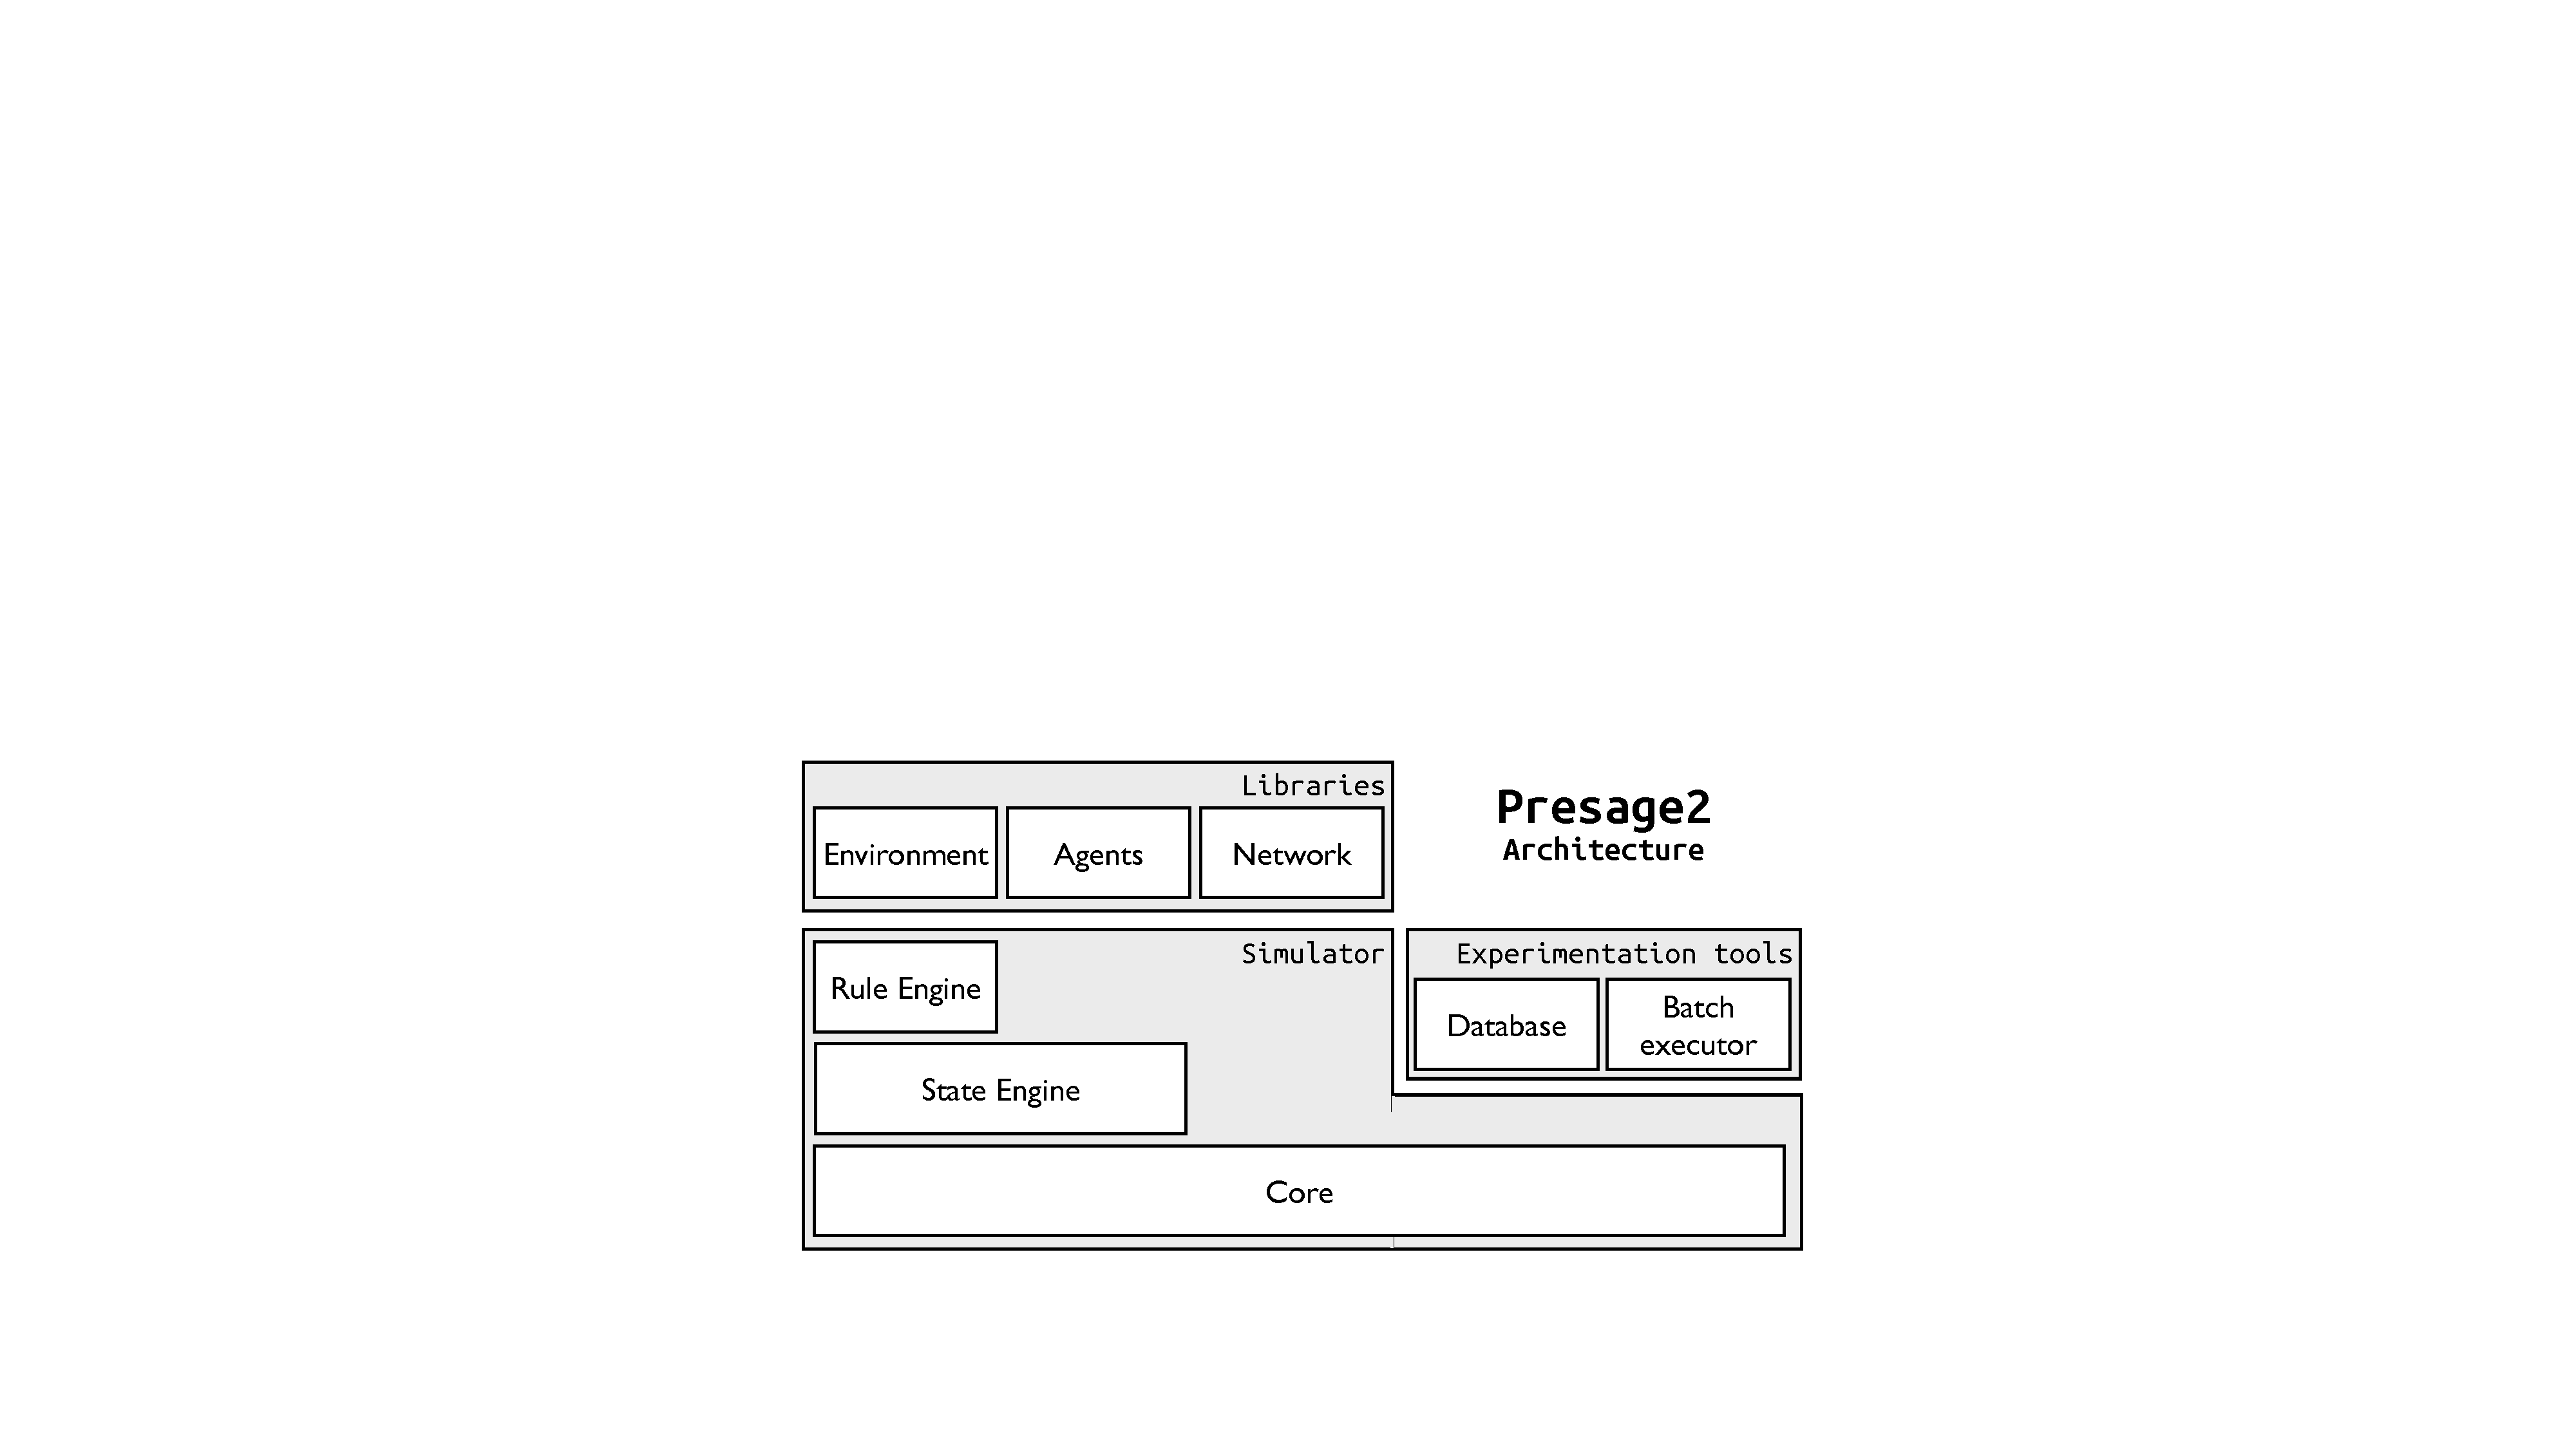
\includegraphics[width=\linewidth]{gfx/presage2/architecture_block}
\caption{Presage2 architectural block diagram}\label{fig:presage2block}
\end{figure}

\begin{figure}
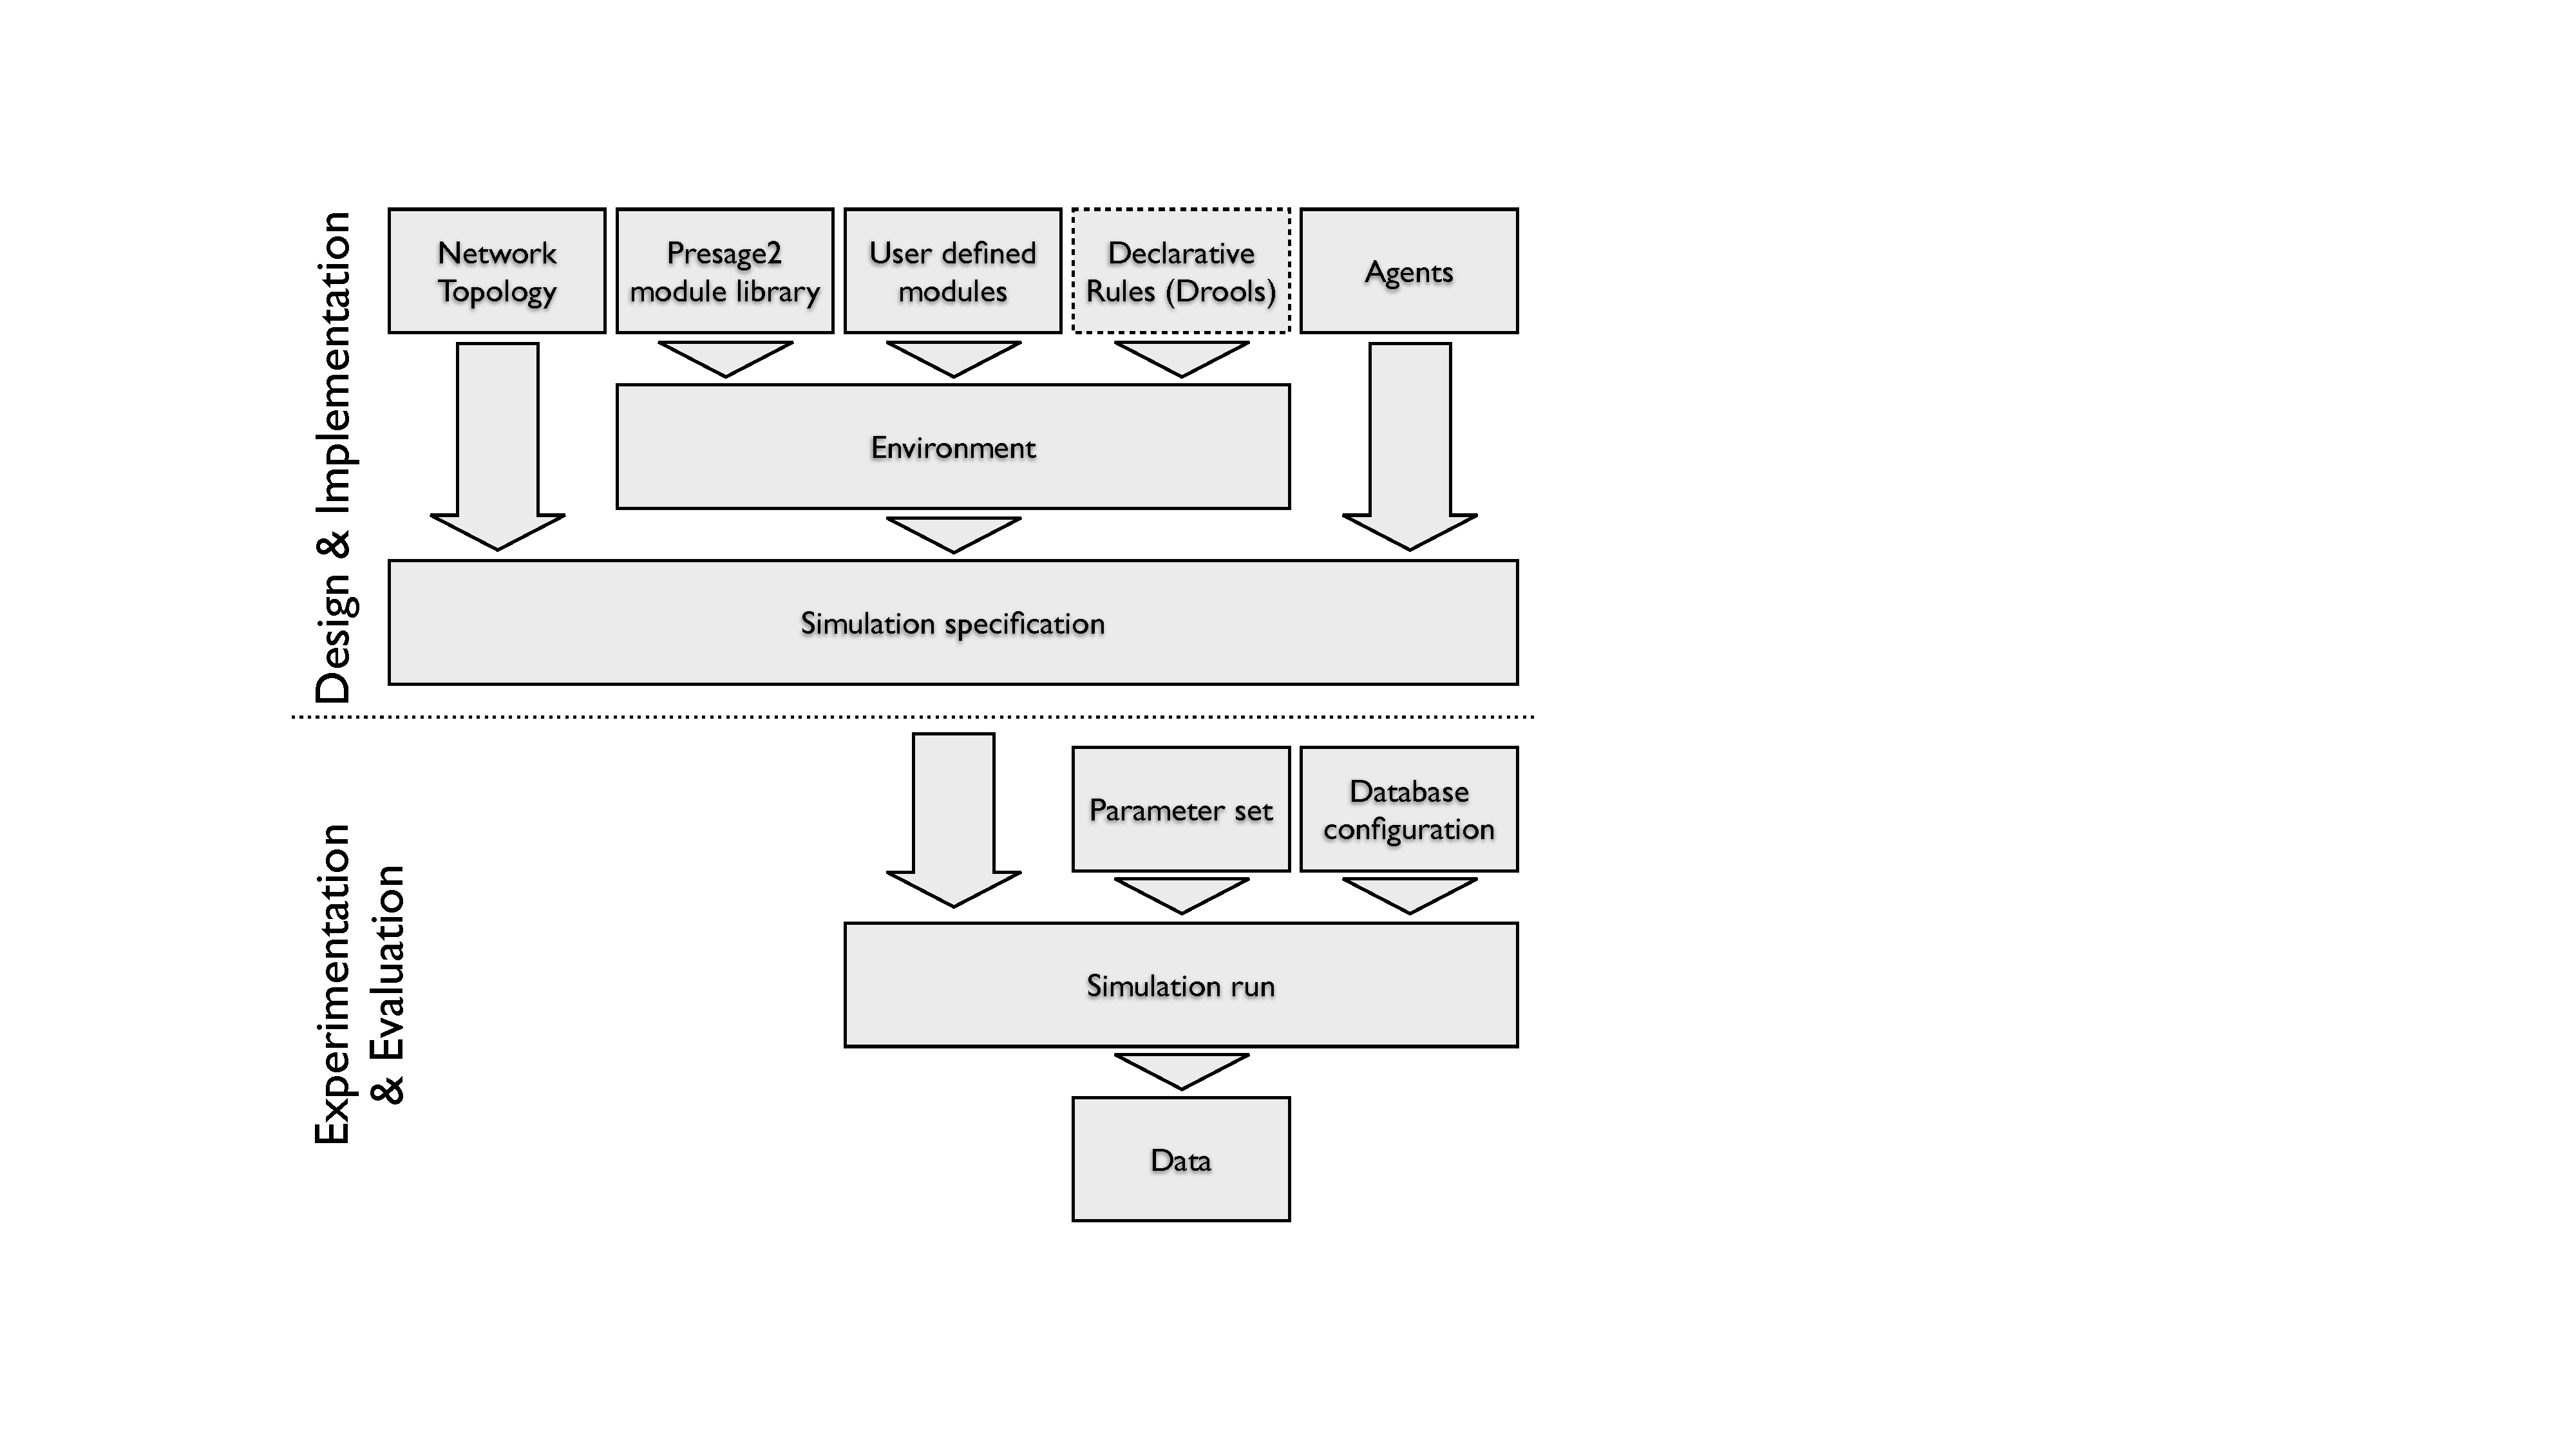
\includegraphics[width=\linewidth]{gfx/presage2/simulation_process}
\caption{Presage2 simulation process diagram}\label{fig:presage2block}
\end{figure}

% Environment requirements
% Agent requirements

%Executable specifications such as the Event Calculus~\citep{Kowalski1986} can even eliminate this step by being both formal representation and computer model~\citep{Artikis2010}. However this approach has limitations in scalability and its ability to span the entire system specification.